
 % !TEX spellcheck = en_US
% !TeX root = main.tex

\begin{figure}[t]
	\centering
	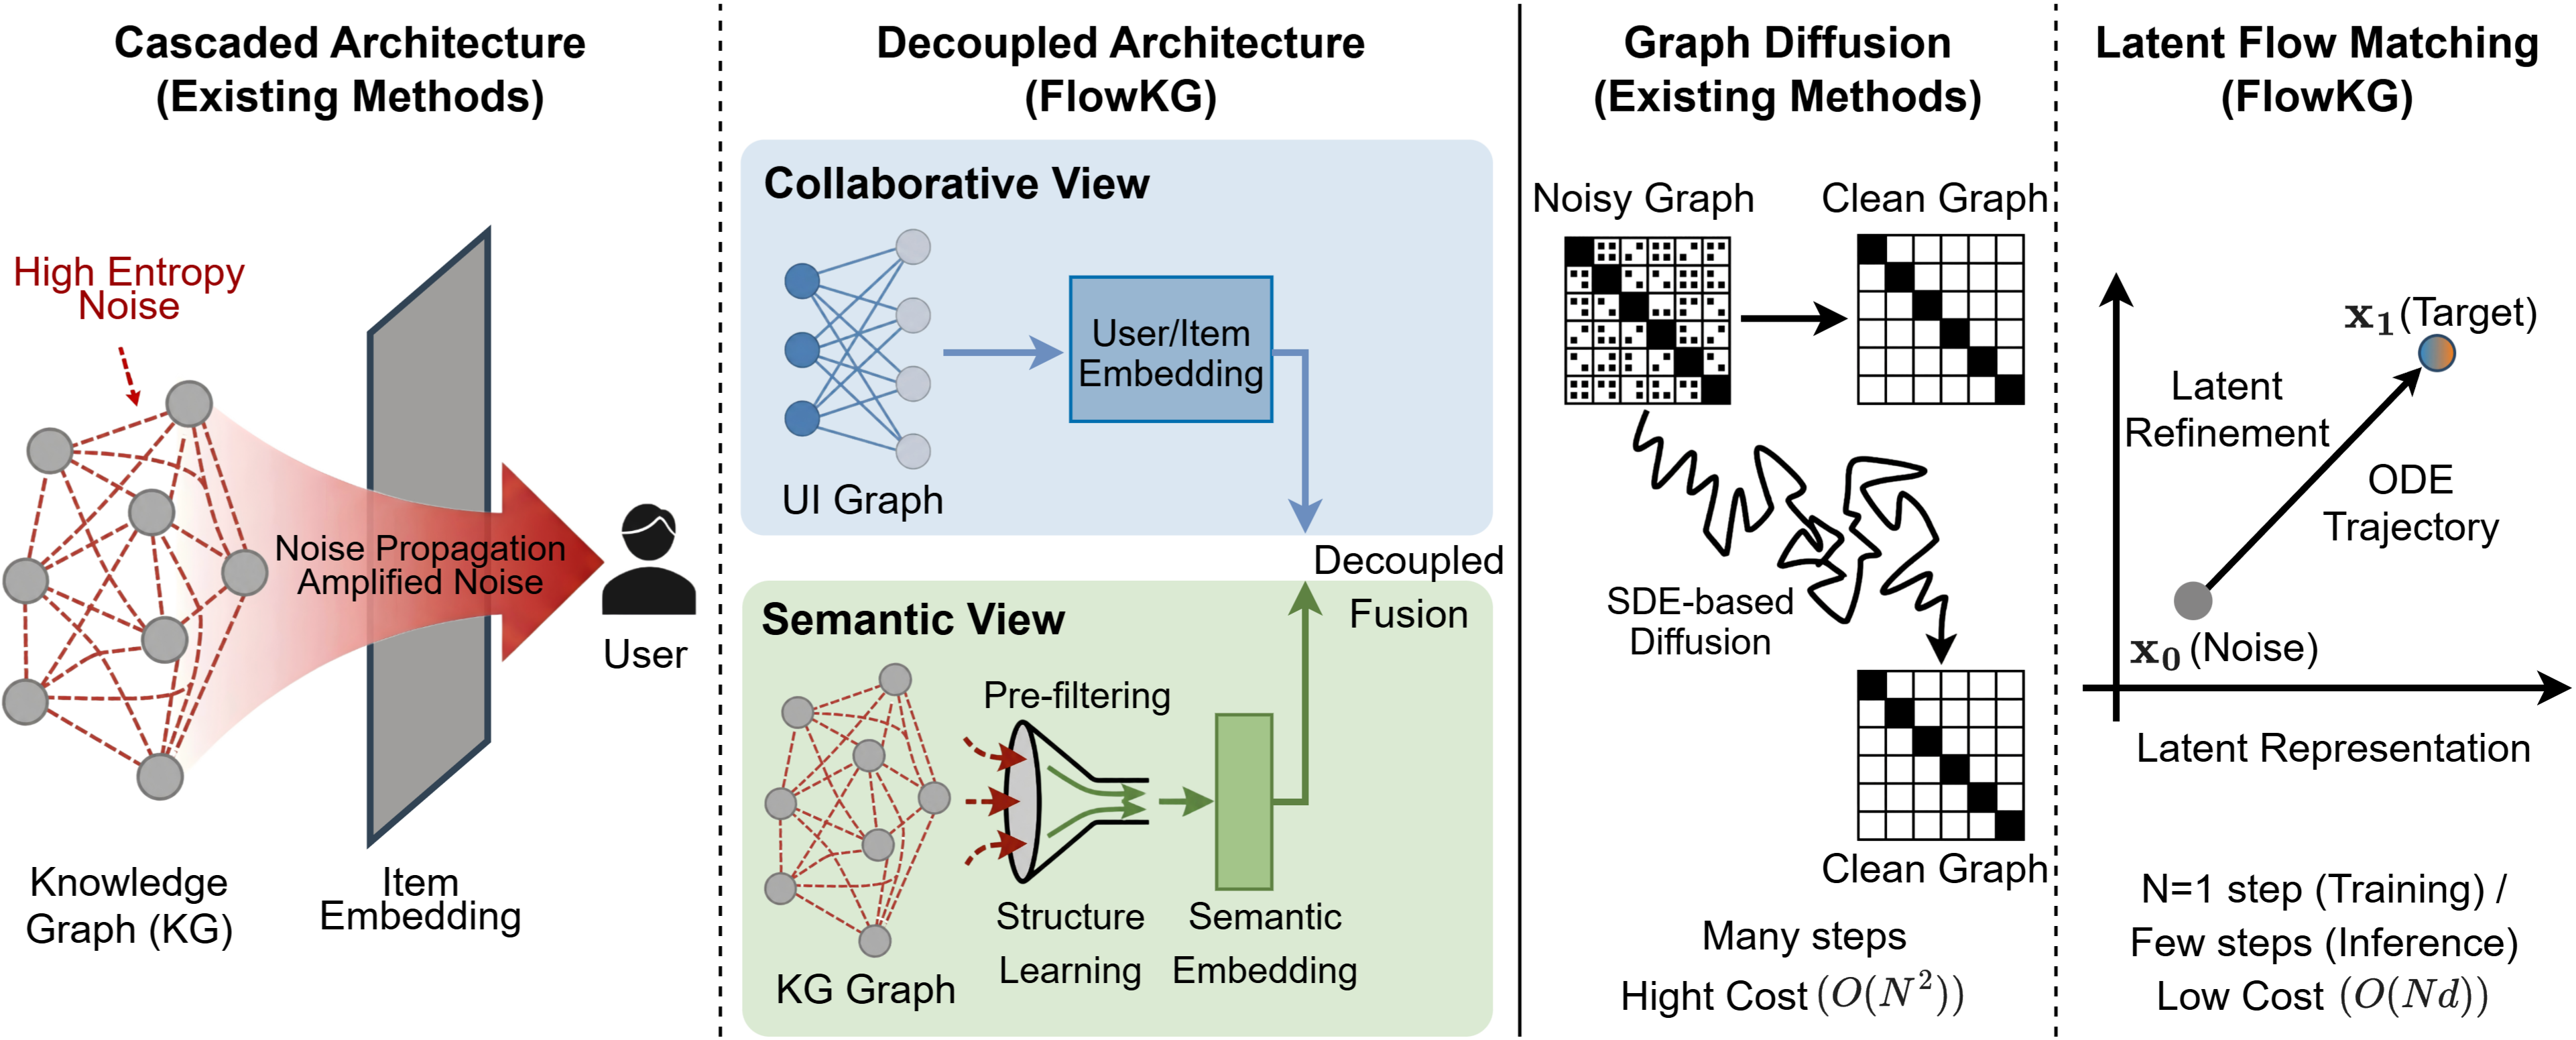
\includegraphics[width=\columnwidth]{image/motivation.png}
	\caption{\textbf{Motivation for FlowKG.} Left: Noise propagation issues. Right: The shift to ODE-based refinement.}
	\label{fig:motivation_main}
\end{figure}


In the era of information explosion, personalized recommender systems serve as pivotal tools for mitigating information overload~\cite{adomavicius2005toward,ricci2010introduction}. To mitigate long-standing challenges such as data sparsity and the cold-start problem, incorporating knowledge graphs (KGs) as auxiliary information has become a common practice~\cite{guo2020survey,zhang2016collaborative}. By mapping items to entities within a structured graph, KGs provide rich semantic connectivity (e.g., Movie-Director, Product-Brand), enabling models to reason about user preferences through high-order relations~\cite{wang2019kgat,wang2018ripplenet}.

Building upon this, Graph Neural Networks (GNNs)~\cite{wang2019kgat, wang2021learning}, renowned for their powerful ability to model graph structures, have achieved notable success in recommendation tasks. However, most existing methods adopt a  ``Cascaded Architecture'': item representations are first enriched by aggregating information from the KG and are then propagated through the user-item interaction graph for collaborative filtering. This tightly-coupled design harbors a critical flaw---noise propagation. Real-world KGs often contain numerous ``one-to-many'' high-entropy connections. For instance,  a single movie might be associated with dozens of generic tags (e.g., classic, emotional). Within a cascaded architecture, as illustrated in Figure~\ref{fig:motivation_main} (Left), such structural noise  is amplified through representation propagation, ultimately contaminating the modeling of user preferences and leading to degraded performance.

To sever this noise propagation pathway, we first propose a fundamental architectural shift: a Decoupled Dual-View Encoder. Unlike cascaded models that subordinate the collaborative signal to the semantic signal, our method processes the Collaborative View (user-item interaction graph) and the Semantic View (KG) in parallel. This design structurally insulates the collaborative learning process from direct structural interference by graph noise, allowing the model to extract clean user behavioral patterns.

Nevertheless, architectural decoupling represents only a partial solution. While it effectively severs the noise propagation path, it does not inherently address the persistent challenge of data sparsity. To combat this, modern recommenders rely on Contrastive Learning (CL)~\cite{yang2022knowledge, zou2022improving} to maximize the mutual information between views. Yet, the efficacy of CL is strictly bound by the quality of the underlying views. If the semantic view remains noisy, standard stochastic augmentations (e.g., random edge dropout) merely yield ``noisy augmented views,'' potentially enforcing the alignment of erroneous semantics. To remedy this, we introduce an Entropy-Guided Structure Learning (ESL) module at the upstream stage. By leveraging relational entropy as a structural prior, ESL identifies and prunes high-uncertainty connections before encoding and augmentation. This ensures that the self-supervised signals in CL are derived from a purified, high-fidelity structure.

Furthermore, even with a purified structure, GNN-based encoders face the inherent limitation of over-smoothing~\cite{li2018deeper,oonograph}, often yielding item representations with limited discriminative power. While recent Generative Recommendation methods (e.g., Diffusion Models~\cite{jiang2024diffkg, li2025mask}) attempt to reconstruct better distributions, they predominantly operate via ``Graph-Level Diffusion'' using Stochastic Differential Equations (SDEs). This paradigm is computationally demanding and indirect, as it generates discrete graph structures rather than optimizing the embeddings themselves. To address this, we introduce a Flow Matching Refinement module at the downstream stage. As shown in Figure~\ref{fig:motivation_main} (Right), we shift from graph diffusion to Latent Representation Refinement. By constructing deterministic Ordinary Differential Equation (ODE) paths based on Optimal Transport, we directly and efficiently rectify item embeddings, evolving them from a noisy distribution to a robust target semantic manifold.

In summary, we propose FlowKG, a holistic framework that integrates decoupled architecture, upstream structure purification, and downstream representation refinement. The main contributions of this work can be summarized  as follows:

\begin{itemize}
	\item \textbf{Novel Architecture:} We identify the noise propagation issue in cascaded architectures and propose a Decoupled Dual-View Encoder to process semantic and collaborative signals in parallel, effectively preventing mutual interference.
	\item \textbf{Methodological Innovation:} We propose a two-stage denoising paradigm: (1) Upstream Entropy-Guided Structure Learning (ESL) to purify the graph structure before contrastive augmentation, and (2) Downstream Flow Matching Refinement to efficiently rectify latent item representations via deterministic ODE paths.
	\item \textbf{SOTA Performance:} Extensive experiments on four benchmark datasets demonstrate that FlowKG significantly outperforms state-of-the-art baselines. The results validate its robustness against noise, as well as its superior training efficiency.
\end{itemize}

